\subsection{サムネイル選択手法の定量比較}

これまでの考察では、採用した平均ヒストグラム法と中央フレーム法の違いを定性的に
述べた。本節ではこれを定量比較に拡張し、代表フレーム選択の 4 手法を同一動画に
適用して、選択結果・評価値の推移・指標間の相互評価・計算時間を比較する。
実験には追加スクリプト {\tt exp01\_thumbnail.py}(付録参照)を用いた。
対象は課題 2 と同じ People - 84973.mp4(1280 $\times$ 720 画素、25 fps、
241 フレーム)であり、実行環境は OpenCV 4.12.0、NumPy 2.4.4 である。

\subsubsection{比較手法と評価指標の定義}

フレーム番号を $i$($i = 0, 1, \dots, 240$)、総フレーム数を $N = 241$ と書く。
比較した手法は以下の 4 つである。

第一の中央フレーム法は、フレームの内容を評価せずに
$\lfloor N/2 \rfloor = 120$ 番のフレームを選ぶ。
第二の平均ヒストグラム法は課題 2 で採用した手法であり、
{\tt task2\_thumbnail\_frame} と同一のロジックで、
{\tt sample\_step} $= 5$ で間引いたフレーム集合
$\mathcal{S} = \{0, 5, \dots, 240\}$(49 フレーム)の各フレームについて
64 ビンのグレースケール正規化ヒストグラム $h_i$ を計算し、
式 \ref{eq:b1-histdist} の評価値 $d_i$ が最小のフレームを選ぶ。

\begin{equation}\label{eq:b1-histdist}
d_i = \left\| h_i - \bar{h} \right\|_2 , \qquad
\bar{h} = \frac{1}{|\mathcal{S}|} \sum_{j \in \mathcal{S}} h_j
\end{equation}

ここで $h_i$ は 64 次元のヒストグラムベクトル、$\bar{h}$ はその平均である。
第三の鮮明度法は、ぼけの少ないフレームほど高周波成分が多く残ることを利用し、
グレースケール画像 $I_i$ にラプラシアンフィルタを適用した結果の分散
(式 \ref{eq:b1-lapvar})が最大のフレームを選ぶ。

\begin{equation}\label{eq:b1-lapvar}
S_i = \mathrm{Var}\left[ \nabla^2 I_i \right]
\end{equation}

$\nabla^2 I_i$ の計算には {\tt cv2.Laplacian} を用いた。
第四のカラフルネス法は、Hasler--Suesstrunk のカラフルネス指標
(式 \ref{eq:b1-colorfulness})が最大のフレームを選ぶ。

\begin{equation}\label{eq:b1-colorfulness}
M_i = \sqrt{\sigma_{rg}^2 + \sigma_{yb}^2}
      + 0.3 \sqrt{\mu_{rg}^2 + \mu_{yb}^2} , \qquad
rg = R - G , \quad yb = \frac{R + G}{2} - B
\end{equation}

ここで $R$、$G$、$B$ は各画素の色成分、$\mu$ と $\sigma$ はそれぞれ
$rg$、$yb$ の画像内での平均と標準偏差である。$M_i$ は彩度の豊かさを
1 つの実数に要約する指標であり、値が大きいほど色鮮やかである。
鮮明度法とカラフルネス法は全 241 フレームを評価対象とした。

\subsubsection{選択フレームと評価値の推移}

表 \ref{tab:b1-selected} に各手法の選択フレームと計算時間を、
図 \ref{fig:b1-traces} に各評価値の全フレームにわたる推移と選択位置を、
図 \ref{fig:b1-frames} に選択されたフレーム画像を示す。

\begin{table}[htbp]
\centering
\caption{各手法の選択フレームと計算時間(People - 84973.mp4、全 241 フレーム)}
\label{tab:b1-selected}
{\small
\begin{tabular}{lrrrr}
\hline
手法 & 選択フレーム & 評価フレーム数 & 総計算時間 [s] & 1 フレームあたり [ms] \\
\hline
中央フレーム法 & 120 & --- & $1 \times 10^{-6}$ & --- \\
平均ヒストグラム法(採用) & 185 & 49 & 4.84 & 98.8 \\
鮮明度法 & 208 & 241 & 6.06 & 25.1 \\
カラフルネス法 & 8 & 241 & 11.73 & 48.7 \\
\hline
\end{tabular}
}
\end{table}

4 手法の選択フレームは 8、120、185、208 とすべて異なった。同一の動画に
対しても、選択基準を変えるだけでサムネイルが完全に入れ替わることが
定量的に確認できた。

図 \ref{fig:b1-traces} (b) より、採用手法の評価値 $d_i$ は動画冒頭
(最大値 0.0207 はフレーム 10)と末尾で大きく、フレーム 170〜190 付近で
小さい。最小値 0.00706 はフレーム 185 で得られ、最小値の 5\% 以内に入る
フレームは 185 と 186 の 2 枚のみであり、選択は明確に定まっている。
(c) のラプラシアン分散 $S_i$ は大部分のフレームで 215〜230 の範囲にあり、
最小値 194.3 は最終フレーム 240 で生じた。最大値 230.1 を与えるフレーム 208
が鮮明度法の選択である。(d) のカラフルネス指標 $M_i$ は動画中盤
(最小値 27.48 はフレーム 78)で低く、冒頭と後半で高い。最大値 28.24 を
与えるフレーム 8 がカラフルネス法の選択である。

図 \ref{fig:b1-frames} の 4 枚はいずれも同一ショット内の画像であり
構図は類似するが、人物の配置と逆光の強さが異なる。フレーム 185 は
課題 2 で出力したサムネイルそのものである。

\begin{figure}[htbp]
\centering
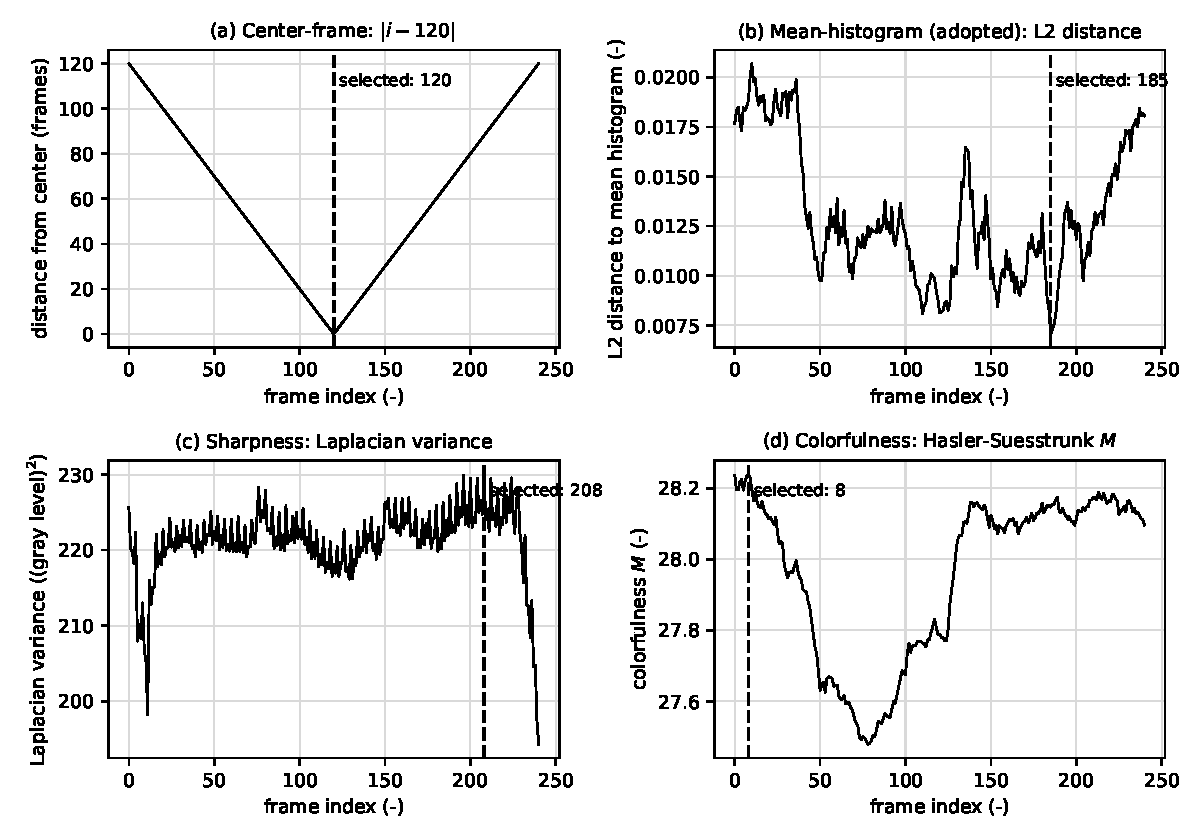
\includegraphics[width=0.92\textwidth]{../experiments/figures/exp01_metric_traces.pdf}
\caption{4 手法の評価値の全フレーム推移。(a) 中央フレーム法(中央からの
距離 $|i - 120|$)、(b) 平均ヒストグラム法(平均ヒストグラムへの L2 距離
$d_i$)、(c) 鮮明度法(ラプラシアン分散 $S_i$)、(d) カラフルネス法
(Hasler--Suesstrunk 指標 $M_i$)。縦の破線は各手法の選択フレーム位置を示す。}
\label{fig:b1-traces}
\end{figure}

\begin{figure}[htbp]
\centering
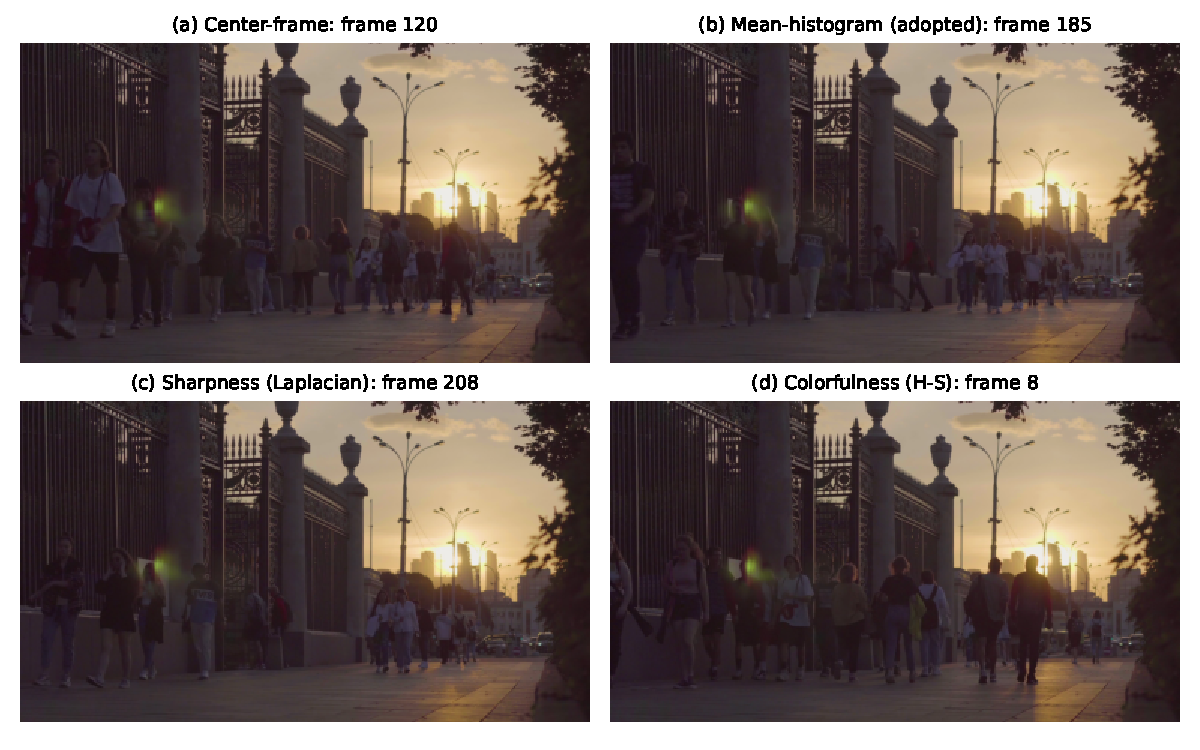
\includegraphics[width=0.95\textwidth]{../experiments/figures/exp01_selected_frames.pdf}
\caption{各手法が選択したフレーム画像。(a) 中央フレーム法(フレーム 120)、
(b) 平均ヒストグラム法(フレーム 185)、(c) 鮮明度法(フレーム 208)、
(d) カラフルネス法(フレーム 8)。}
\label{fig:b1-frames}
\end{figure}

\subsubsection{指標間の相互評価}

各手法の選択フレームを、他の手法の評価指標でも採点した結果を
表 \ref{tab:b1-cross} に示す。表中の百分位は、全 241 フレーム中で当該値
以下のフレームが占める割合であり、$d_i$ は小さいほど、$S_i$ と $M_i$ は
大きいほど良い値である。

\begin{table}[htbp]
\centering
\caption{各手法の選択フレームにおける 3 指標の値と百分位。百分位は
全 241 フレーム中で当該値以下のフレームが占める割合 [\%] を表す。}
\label{tab:b1-cross}
{\small
\begin{tabular}{lrrrrrrr}
\hline
手法 & フレーム & $d_i$ & 百分位 & $S_i$ & 百分位 & $M_i$ & 百分位 \\
\hline
中央フレーム法 & 120 & 0.00814 & 2.5 & 218.2 & 14.9 & 27.79 & 30.7 \\
平均ヒストグラム法(採用) & 185 & 0.00706 & 0.4 & 221.2 & 44.8 & 28.15 & 78.0 \\
鮮明度法 & 208 & 0.01101 & 31.5 & 230.1 & 100.0 & 28.17 & 89.2 \\
カラフルネス法 & 8 & 0.01882 & 92.9 & 213.0 & 6.2 & 28.24 & 100.0 \\
\hline
\end{tabular}
}
\end{table}

採用手法が選んだフレーム 185 は、$d_i$ が全フレーム最小(百分位 0.4\%)で
あることに加えて、鮮明度 $S_i$ の百分位 44.8\%(ほぼ中央値)、カラフルネス
$M_i$ の百分位 78.0\% と、最適化の対象としていない指標でも中位以上の値を
示した。すなわち、明るさ分布の代表性を基準に選んだフレームが、鮮明度・
彩度の面でも大きな欠点を持たないことが確認できた。

中央フレーム 120 の $d_i$ は 0.00814 で、最小値より 15.3\% 大きいだけで
ある(百分位 2.5\%)。この動画に限れば中央フレームも明るさ分布の代表性は
高いが、これは本動画が場面転換のない単一ショットで、画面構成が緩やかに
しか変化しないためと考えられる。一方で鮮明度は百分位 14.9\% と下位に
あり、中央フレーム法がフレームの品質を評価しないという欠点は数値にも
表れている。

カラフルネス法が選んだフレーム 8 は、$M_i$ こそ最大(28.24)だが、
$d_i$ の百分位が 92.9\% と明るさ分布が最も非典型的な部類に属し
($d_i$ 最大のフレーム 10 の直近でもある)、鮮明度も百分位 6.2\% と
最もぼけた部類にある。単一指標の最大化は、その指標以外の品質を大きく
犠牲にし得ることを示す実例である。鮮明度法のフレーム 208 は $S_i$ 最大
(230.1)かつ $M_i$ 百分位 89.2\% と良好だが、$d_i$ は百分位 31.5\% に
とどまり、明るさ分布の代表性では採用手法に劣る。

指標としての判別力にも大きな差があった。変動係数(標準偏差を平均で
割った値)は $d_i$ が 25.7\% であるのに対し、$S_i$ は 2.26\%、$M_i$ は
0.83\% にすぎない。特に $M_i$ は全変動幅(最大値と最小値の差)が平均値の
2.7\% しかなく、わずかな差で選択が決まるため、この動画に対する分離能は
乏しい。採用手法の評価値 $d_i$ は相対変動が最も大きく、フレーム間の差を
最も明瞭に区別できる指標であった。

また、3 指標の全フレームにわたる相関は弱く、Pearson 相関係数は
$d_i$--$S_i$ 間で $-0.384$、$d_i$--$M_i$ 間で $+0.332$、$S_i$--$M_i$ 間で
$-0.086$、Spearman 順位相関係数はそれぞれ $-0.161$、$+0.314$、$+0.053$
であった。図 \ref{fig:b1-normalized} に min--max 正規化した 4 つの評価値を
重ねて示すが、極小・極大の位置は指標ごとに異なる。3 指標は互いにほぼ独立
した性質(代表性・鮮明度・彩度)を測っており、単一指標で他を代替する
ことはできない。したがって、サムネイルの総合品質をさらに高めるには、
複数指標の重み付き結合が改善方向となる。

\begin{figure}[htbp]
\centering
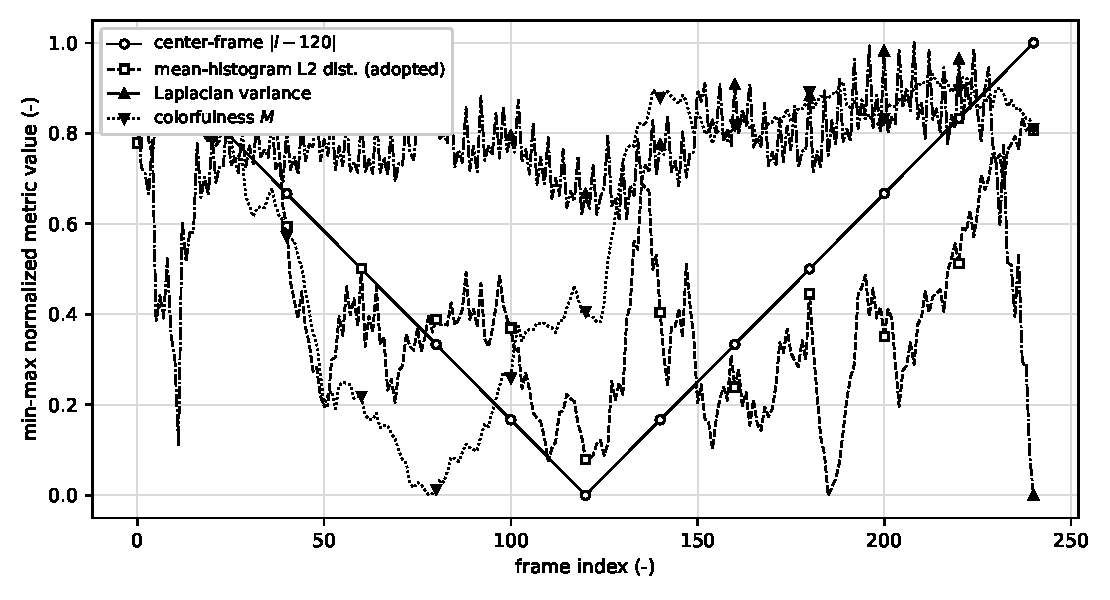
\includegraphics[width=0.88\textwidth]{../experiments/figures/exp01_normalized.pdf}
\caption{min--max 正規化した 4 手法の評価値の重ね描き。中央からの距離
$|i - 120|$ と $d_i$ は小さいほど、$S_i$ と $M_i$ は大きいほど良い値である。}
\label{fig:b1-normalized}
\end{figure}

\subsubsection{サンプリング間隔と計算時間}

採用手法の {\tt sample\_step} $= 5$ の妥当性も検証した。全フレームを
評価に用いた場合({\tt sample\_step} $= 1$)の選択もフレーム 185 で
一致し、間引きによる選択の変化は 0 フレームであった。すなわち、この動画
では評価フレーム数を 241 枚から 49 枚へ 1/5 に減らしても選択結果は変わらず、
間引きは計算量削減の手段として妥当である。

計算時間は表 \ref{tab:b1-selected} のとおりである。中央フレーム法は
添字計算のみで約 $10^{-6}$ s と事実上ゼロである。内容に基づく 3 手法では、
採用手法が 4.84 s と最も短く、鮮明度法(6.06 s)の 79.9\%、カラフルネス法
(11.73 s)の 41.3\% であった。ただし 1 フレームあたりの指標計算は採用手法
が 98.8 ms と最も重く(鮮明度法 25.1 ms の 3.9 倍、カラフルネス法 48.7 ms
の 2.0 倍)、総時間が最短になるのは間引きの効果である。ヒストグラム計算に
汎用の {\tt numpy.histogram} を用いていることが 1 フレームあたりの時間を
押し上げており、OpenCV の専用関数 {\tt cv2.calcHist} に置き換えることで
短縮できると考えられる。なお、動画のデコードには全手法共通で 4.64 s
(241 フレーム、19.3 ms/フレーム)を要しており、内容に基づく選択手法の
実行時間はデコード時間と同程度以上になる点も設計上考慮すべきである。

\subsubsection{キーフレーム抽出研究における位置付け}

動画要約の近年のサーベイ \cite{b1-tiwari2021} では、キーフレームは動画を
代表する最も重要なフレームと定義され、静的要約(サムネイルを含む)の生成
では色などの低水準特徴の変化に基づく抽出が基本的な構成要素とされている。
採用した平均ヒストグラム法は、この分類における低水準特徴(明るさ分布)の
代表性基準に相当する。また、深層学習に基づく動画要約のサーベイ
\cite{b1-apostolidis2021} が扱うように、近年は代表性や多様性を学習によって
最適化する手法が発展しているが、これらは学習データと計算資源を要する。
本課題のように単一動画から 1 枚のサムネイルを選ぶ用途では、本実験で示した
とおり、低水準特徴による選択でも鮮明度・彩度の百分位がそれぞれ 44.8\%・
78.0\% と均衡の取れたフレームが得られる。

以上より、採用手法は(1)評価値の変動係数が 25.7\% と最も大きく判別力に
優れること、(2)最適化の対象外の指標でも中位以上の値を示し極端な欠点が
ないこと、(3)内容に基づく 3 手法の中で計算時間が最短であることの 3 点
から、比較した手法の中で最も妥当なサムネイル選択基準であると結論できる。
